\section{Figure excerpts from documentation sources}
\begin{figure}[H]
    \centering
    \begin{subfigure}[b]{0.5\textwidth}
         \centering
         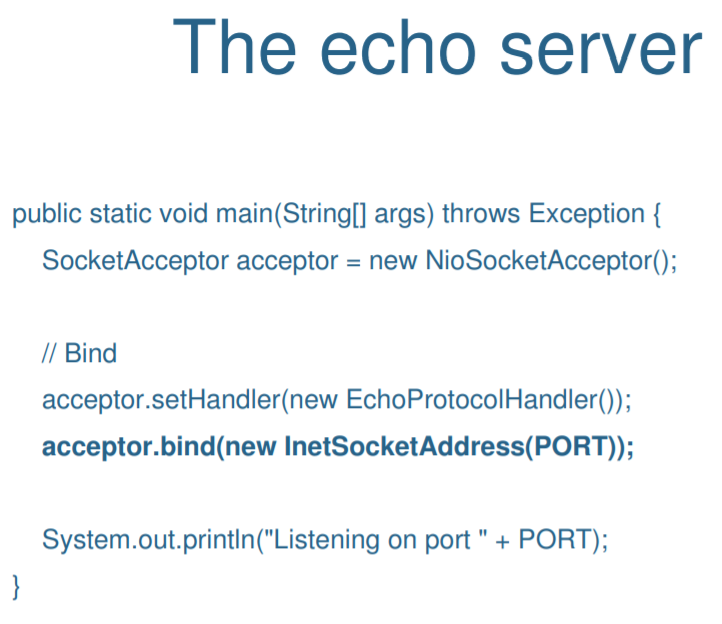
\includegraphics[width=\textwidth]{images/usability_extensibility1.png}
     \end{subfigure}
   
     \begin{subfigure}[b]{0.5\textwidth}
         \centering
         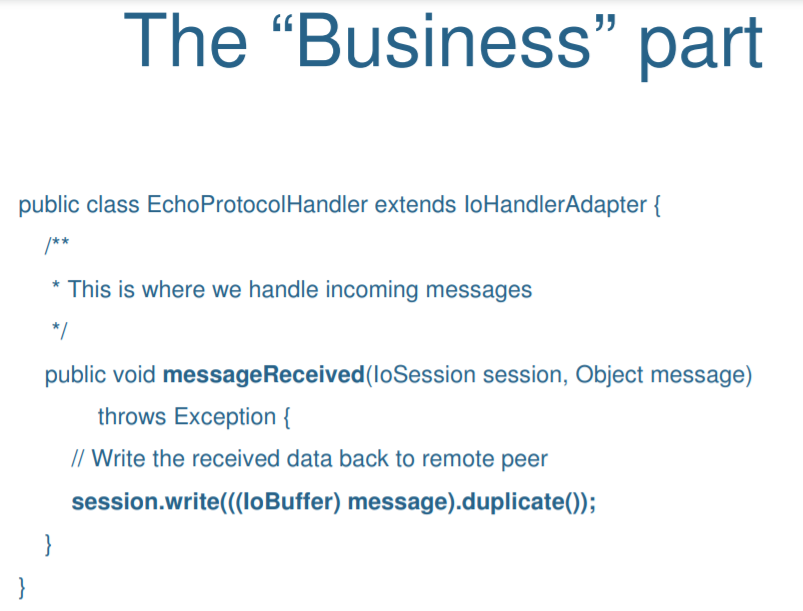
\includegraphics[width=\textwidth]{images/usability_extensibility2.png}
     \end{subfigure}
   
    \begin{subfigure}[b]{0.5\textwidth}
         \centering
         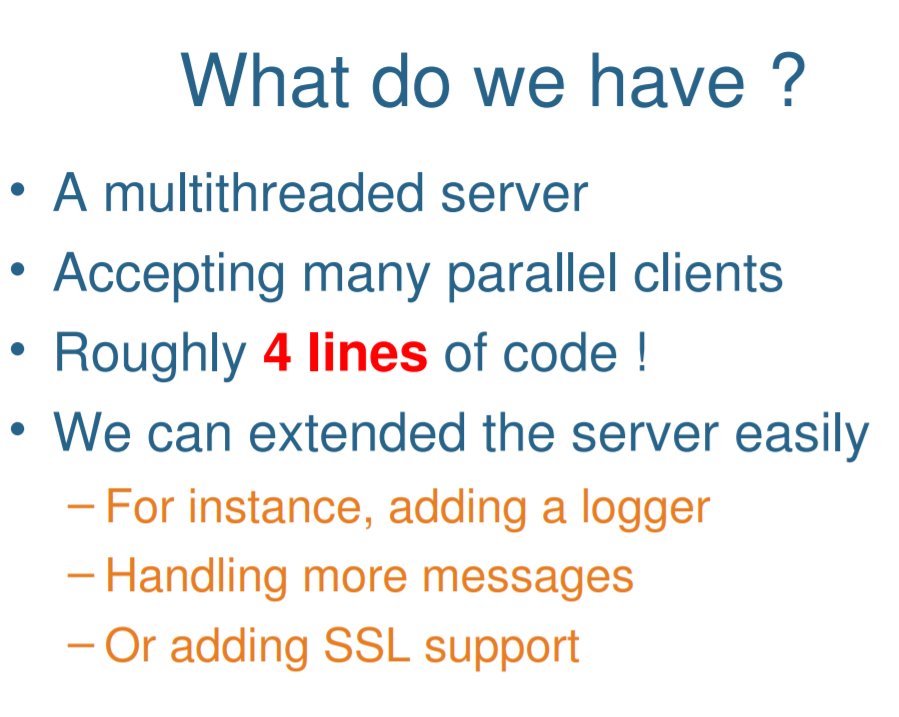
\includegraphics[width=\textwidth]{images/usability_extensibility.png}
     \end{subfigure}
    
    \caption{An exercept from \cite{mina-talk2009} that showcases the ease of use and extensibility of the MINA framework.}
    \label{fig:usability_extensibility}
\end{figure}

\begin{figure}[H]
    \centering
    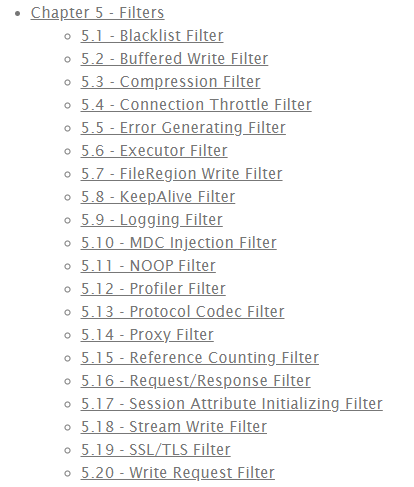
\includegraphics[width=0.6\textwidth]{images/filters.png}
    \caption{An overview of the out-of-the-box filters offered by the MINA framework; the overview has been extracted from \cite{mina-userguide}.}
    \label{fig:filters}
\end{figure}

\begin{figure}[H]
    \centering
    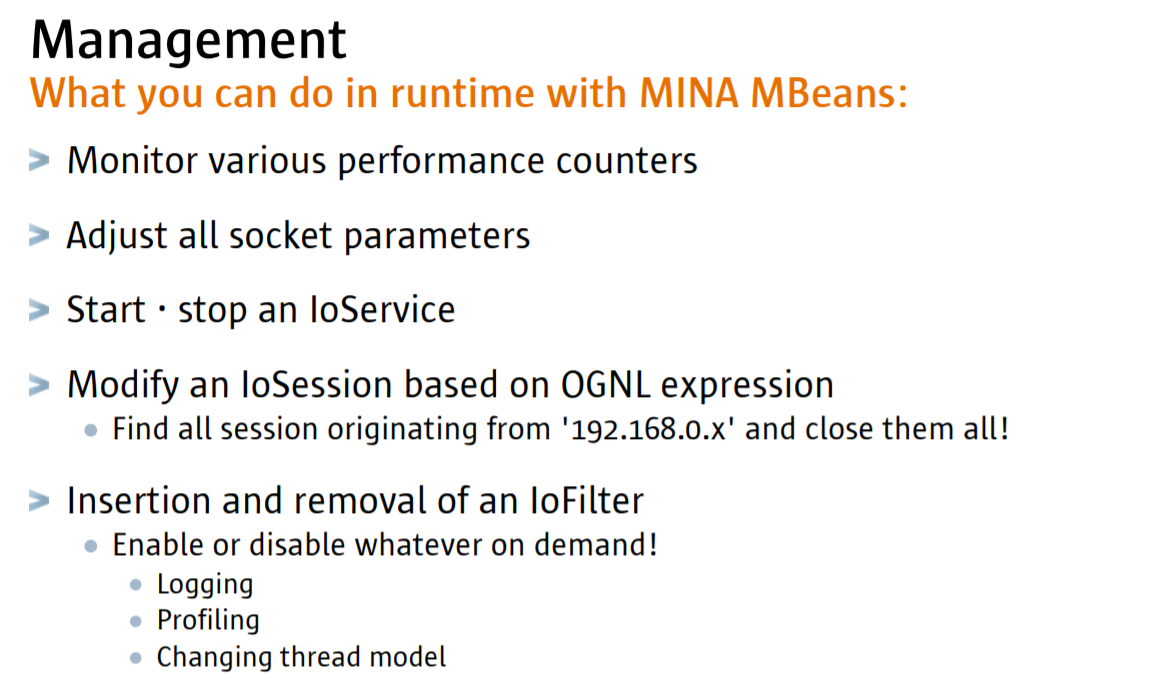
\includegraphics[width=0.7\textwidth]{images/management.png}
    \caption{Excerpt from \cite{mina-talk2008} showing the runtime management capabilities of MINA applications integrated with JMX.}
    \label{fig:manageability}
\end{figure}

\begin{figure}[H]
    \centering
    \begin{subfigure}[b]{0.7\textwidth}
         \centering
         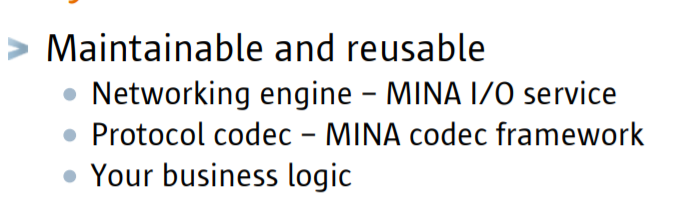
\includegraphics[width=\textwidth]{images/reusable1.png}
     \end{subfigure}

     \begin{subfigure}[b]{0.7\textwidth}
         \centering
         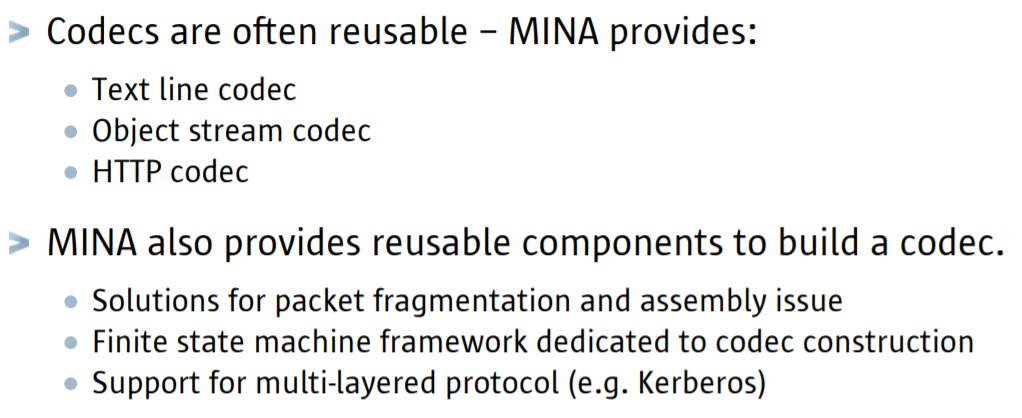
\includegraphics[width=\textwidth]{images/reusable.png}
     \end{subfigure}
     
    \begin{subfigure}[b]{0.7\textwidth}
         \centering
         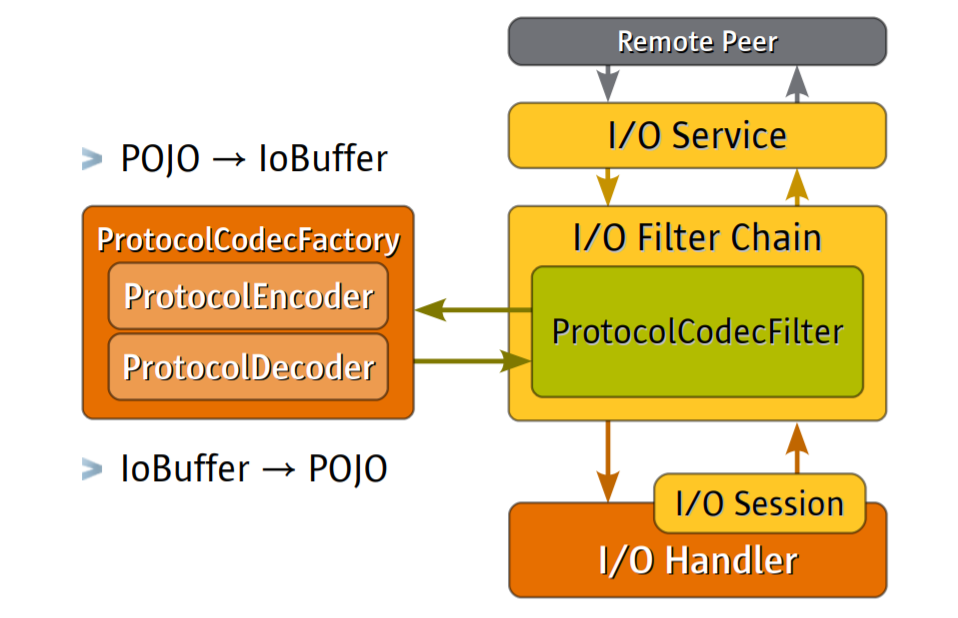
\includegraphics[width=\textwidth]{images/architecture_codec.png}
     \end{subfigure}
    
    \caption{An exercept from the presentation \cite{mina-talk2008} that showcases the high reusability  of components from the MINA framework.}
    \label{fig:reusability}
\end{figure}

